%!TEX TS-program = lualatex
%!TEX encoding = UTF-8 Unicode

%\frame[plain]{ % When including a large figure or table, you don't want to have the bottom and the top of the slides.
%\frame[shrink]{ % If you want to include lots of text on a slide, use the shrink option.


\begin{frame}[plain]
    \frametitle{Throughput Relative to Linux Loopback Mounting}
    \vspace*{-1pt}
    \makebox[\linewidth]{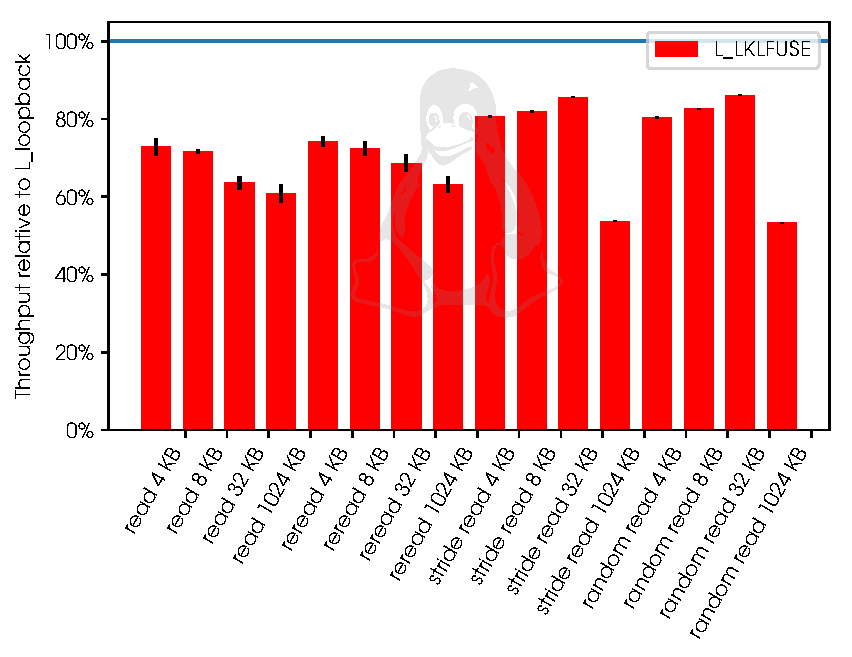
\includegraphics[page=1,width=0.87\paperwidth]{frames/img/relative_performance_filter_read_baseline_L_loopback_variants_L_LKLFUSE}}
    \note{
        \begin{itemize}
            \item blue line is baseline, mounting FS via Linux Kernel
            \item Y-access LKLFUSE relative to baseline loopback-mounting
            \item X-axis, workloads
            \item LKLFUSE delivers okay read performance, i.e. 72\%
            \item very consistent irregardless of blocksize. readahead
        \end{itemize}
    }
\end{frame}

\begin{frame}[plain]
\frametitle{Throughput Relative to Linux Loopback Mounting}
\vspace*{-1pt}
\makebox[\linewidth]{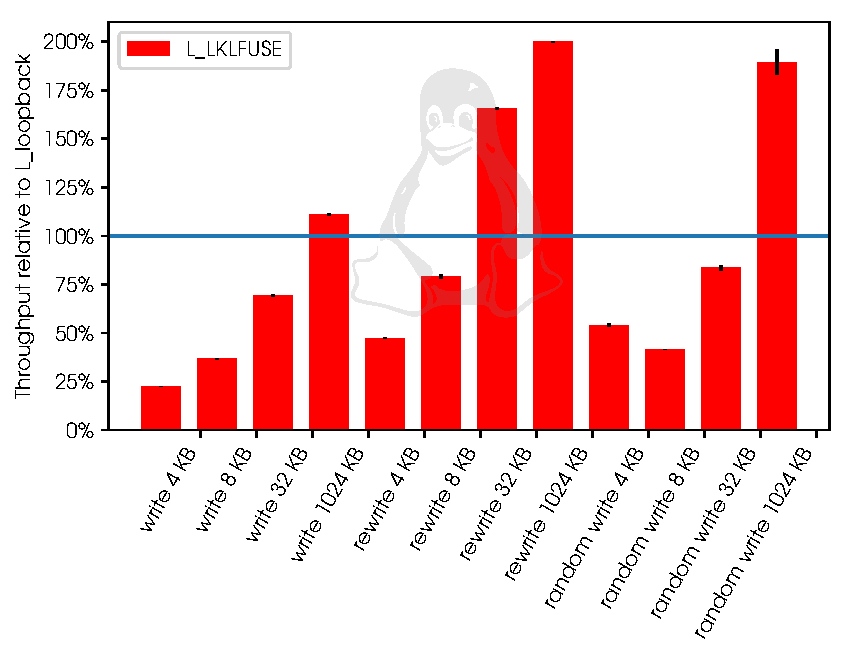
\includegraphics[page=1,width=0.87\paperwidth]{frames/img/relative_performance_filter_write_baseline_L_loopback_variants_L_LKLFUSE}}
\note{
    \begin{itemize}
        \item LKLFUSE: seq write delivers okay performance, i.e. above 50\%
        \item big difference between blocksizes. Overhead of each write reaching the FS one by one
        \item much better than baseline: how is that possible?
        \item writing to pages that have not been written back (rewrite, random write), writeback caching
        \item multiple layers of caching
    \end{itemize}
}
\end{frame}
